\documentclass[10pt,twocolumn,letterpaper]{article}
\usepackage[margin=0.75in,columnsep=0.28in]{geometry}
\usepackage{newtxtext,newtxmath}
\usepackage[T1]{fontenc}
\usepackage{microtype,graphicx,booktabs,longtable,caption,subcaption,xcolor,enumitem,amsmath}
\usepackage[hidelinks]{hyperref}
\usepackage{titlesec,float}
\captionsetup{font=small,labelfont=bf}
\titleformat{\section}{\large\bfseries}{\thesection}{0.6em}{}
\titleformat{\subsection}{\normalsize\bfseries}{\thesubsection}{0.6em}{}
\setlist{nosep,leftmargin=1.2em}
\definecolor{oski}{HTML}{3F7D58}
\newcommand{\figw}{\columnwidth}
\newcommand{\sessiontable}{%
\begin{table*}[t]\centering\small
\caption{The five observed sessions. Face px: median face size. Camera: share of the recording with $\geq$3 faces in view. Recognised: students named for $\geq$3\,s; glimpsed: named for under 3\,s. Wrong sec.: people matched from another section (certain errors, any duration). Minutes of instructor and non-instructor speech from voiceprints. Calls: instructor name calls detected. Named: student comments attributed.}
\label{tab:sessions}
\resizebox{\textwidth}{!}{\begin{tabular}{lrrrrrrrrrr}\toprule
Class & Video & Face px & Camera & Recognised & Glimpsed & Wrong sec. & Instr. min & Student min & Calls & Named\\\midrule
Sep 22 & 1024$\times$576 & 29 & 33\% & 42 & 1 & 1 & 50 & 39 & 10 & 32 \\
Sep 24 & 1024$\times$576 & 30 & 26\% & 41 & 3 & 4 & 52 & 22 & 13 & 30 \\
Sep 29 & 1024$\times$576 & 33 & 22\% & 36 & 1 & 4 & 57 & 26 & 4 & 12 \\
Oct 6 & 1024$\times$576 & 33 & 24\% & 33 & 3 & 0 & 33 & 57 & 4 & 21 \\
Oct 8 & 1920$\times$1080 & 57 & 11\% & 41 & 2 & 1 & 37 & 11 & 3 & 7 \\
\bottomrule\end{tabular}}\end{table*}}

\newcommand{\idtable}{%
\begin{table}[t]\centering\small
\caption{Identification on the 1080p session (5,785 faces $\geq$24\,px, sampled every 2\,s) against a 229-student, four-section gallery. Certain errors are matches to another section; estimated correctness scales them by 229/172.}
\label{tab:id}
\resizebox{\columnwidth}{!}{\begin{tabular}{rrrrrrr}\toprule
$\tau$ & Named & Share & Certain err. & Est.\ correct & Students & Wrong people\\\midrule
0.40 & 2,579 & 44.6\% & 19 & 99.0\% & 44 & 16 \\
0.45 & 2,025 & 35.0\% & 3 & 99.8\% & 43 & 3 \\
0.50 & 1,393 & 24.1\% & 0 & 100.0\% & 42 & 0 \\
0.55 & 765 & 13.2\% & 0 & 100.0\% & 37 & 0 \\
0.60 & 304 & 5.3\% & 0 & 100.0\% & 27 & 0 \\
\bottomrule\end{tabular}}\end{table}}

\newcommand{\vertable}{%
\begin{table}[t]\centering\small
\caption{Verification from the classroom's own footage: 2,733 same-seat pairs (1\,s apart) and 19,801 same-frame pairs. The last column is the chance an unknown face clears the bar against at least one of 70 enrolled students.}
\label{tab:ver}
\begin{tabular}{rrrr}\toprule
$\tau$ & Same person & False match / pair & False match vs 70\\\midrule
0.300 & 99.5\% & 3.596\% & 92.3\% \\
0.363 & 99.2\% & 0.828\% & 44.1\% \\
0.400 & 98.8\% & 0.278\% & 17.7\% \\
0.450 & 97.9\% & 0.081\% & 5.5\% \\
0.500 & 96.9\% & 0.010\% & 0.7\% \\
\bottomrule\end{tabular}\end{table}}

\newcommand{\studenttable}{%
\begin{footnotesize}\setlength{\tabcolsep}{5pt}\renewcommand{\arraystretch}{0.95}
\begin{longtable}{lrrrrrrrrrl}
\caption{Every student, by anonymous id. Seconds recognised on camera per class (``--'' = not recognised), classes present ($\geq$3\,s), named comments ($^\dagger$ includes voice matches from a class the student was not seen in), named talk seconds, times called on, and whether a voiceprint was learned.}\label{tab:students}\\\toprule
Student & Sep 22 & Sep 24 & Sep 29 & Oct 6 & Oct 8 & Cls & Cmts & Talk s & Calls & Voice\\\midrule\endfirsthead
\toprule Student & Sep 22 & Sep 24 & Sep 29 & Oct 6 & Oct 8 & Cls & Cmts & Talk s & Calls & Voice\\\midrule\endhead
S01 & 134 & 25 & 55 & 65 & -- & 4 & 0 & 0 & 1 &  \\
S02 & 404 & 118 & 158 & 177 & 211 & 5 & 0 & 0 & 0 &  \\
S03 & -- & -- & -- & -- & 4 & 1 & 0 & 0 & 1 &  \\
S04 & 342 & 207 & 252 & 477 & -- & 4 & 0 & 0 & 0 &  \\
S05 & -- & -- & -- & -- & 7 & 1 & 9$^\dagger$ & 264 & 1 & yes \\
S06 & -- & 376 & 40 & 26 & 83 & 4 & 0 & 0 & 0 &  \\
S07 & 498 & 117 & 119 & 12 & -- & 4 & 3 & 80 & 2 & yes \\
S08 & 10 & 1 & -- & 406 & 120 & 3 & 0 & 0 & 0 &  \\
S09 & -- & -- & 4 & -- & 78 & 2 & 0 & 0 & 0 &  \\
S10 & 20 & 6 & -- & -- & -- & 2 & 0 & 0 & 0 &  \\
S11 & 31 & 294 & -- & -- & 187 & 3 & 0 & 0 & 0 &  \\
S12 & 540 & 368 & 252 & 317 & 273 & 5 & 9 & 108 & 2 & yes \\
S13 & -- & 65 & 230 & -- & -- & 2 & 0 & 0 & 0 &  \\
S14 & 200 & 144 & 155 & 73 & 262 & 5 & 0 & 0 & 0 &  \\
S15 & 229 & -- & 150 & -- & -- & 2 & 0 & 0 & 0 &  \\
S16 & -- & 2 & 15 & 2 & 103 & 2 & 0 & 0 & 0 &  \\
S17 & 202 & 71 & 22 & 213 & 85 & 5 & 0 & 0 & 0 &  \\
S18 & 399 & 322 & 96 & 12 & 261 & 5 & 0 & 0 & 0 &  \\
S19 & 7 & 286 & 245 & -- & 38 & 4 & 5$^\dagger$ & 117 & 1 & yes \\
S20 & 121 & 213 & 95 & 237 & 238 & 5 & 0 & 0 & 0 &  \\
S21 & -- & 37 & -- & 3 & 44 & 3 & 3$^\dagger$ & 110 & 1 & yes \\
S22 & 2 & -- & -- & 50 & 2 & 1 & 7$^\dagger$ & 190 & 3 & yes \\
S23 & 100 & 129 & 44 & -- & 109 & 4 & 5$^\dagger$ & 94 & 3 & yes \\
S24 & 398 & 378 & 66 & 340 & 171 & 5 & 19 & 492 & 2 & yes \\
S25 & 87 & 348 & -- & 38 & 59 & 4 & 0 & 0 & 0 &  \\
S26 & -- & 324 & 400 & 683 & 105 & 4 & 0 & 0 & 0 &  \\
S27 & -- & 248 & 23 & 28 & 71 & 4 & 0 & 0 & 0 &  \\
S28 & 99 & 212 & -- & 146 & -- & 3 & 0 & 0 & 0 &  \\
S29 & 220 & 66 & -- & -- & 252 & 3 & 8 & 143 & 1 & yes \\
S30 & -- & 250 & -- & 480 & 54 & 3 & 4 & 57 & 1 & yes \\
S31 & 66 & 138 & 110 & 4 & 53 & 5 & 0 & 0 & 0 &  \\
S32 & 145 & 197 & 189 & 68 & 168 & 5 & 0 & 0 & 0 &  \\
S33 & 41 & 74 & 33 & 191 & 10 & 5 & 0 & 0 & 0 &  \\
S34 & -- & -- & -- & -- & -- & 0 & 0 & 0 & 1 &  \\
S35 & 156 & 18 & 124 & 561 & -- & 4 & 0 & 0 & 0 &  \\
S36 & 369 & 108 & 338 & 128 & 159 & 5 & 0 & 0 & 1 &  \\
S37 & 482 & -- & 95 & 203 & -- & 3 & 0 & 0 & 0 &  \\
S38 & 131 & -- & 143 & 246 & 178 & 4 & 0 & 0 & 0 &  \\
S39 & 155 & -- & -- & -- & 7 & 2 & 0 & 0 & 0 &  \\
S40 & -- & -- & -- & -- & -- & 0 & 0 & 0 & 0 &  \\
S41 & 290 & 264 & 84 & -- & 93 & 4 & 9 & 367 & 3 & yes \\
S42 & 281 & 188 & 283 & -- & 78 & 4 & 3 & 80 & 3 & yes \\
S43 & 23 & 50 & 2 & -- & 4 & 3 & 0 & 0 & 0 &  \\
S44 & 20 & 29 & 167 & 2 & 257 & 4 & 0 & 0 & 0 &  \\
S45 & 440 & 201 & -- & -- & 55 & 3 & 0 & 0 & 0 &  \\
S46 & 407 & 262 & 443 & 90 & -- & 4 & 0 & 0 & 0 &  \\
S47 & -- & -- & -- & 58 & 5 & 2 & 0 & 0 & 0 &  \\
S48 & 730 & 161 & -- & -- & 81 & 3 & 6$^\dagger$ & 128 & 3 & yes \\
S49 & -- & -- & -- & -- & 1 & 0 & 2$^\dagger$ & 71 & 1 & yes \\
S50 & 202 & 89 & 71 & -- & 55 & 4 & 3 & 69 & 1 & yes \\
S51 & -- & 75 & -- & 22 & 172 & 3 & 0 & 0 & 0 &  \\
S52 & 79 & 2 & -- & 182 & 168 & 3 & 7 & 150 & 1 & yes \\
S53 & 387 & 27 & 151 & 2 & -- & 3 & 0 & 0 & 0 &  \\
S54 & 385 & -- & 265 & 40 & 190 & 4 & 0 & 0 & 1 &  \\
S55 & 125 & 52 & 378 & 122 & 68 & 5 & 0 & 0 & 0 &  \\
S56 & 184 & -- & -- & -- & -- & 1 & 0 & 0 & 0 &  \\
S57 & 51 & 153 & 355 & 399 & -- & 4 & 0 & 0 & 0 &  \\
S58 & 433 & 134 & 77 & -- & 49 & 4 & 0 & 0 & 0 &  \\
\bottomrule\end{longtable}\end{footnotesize}}

\newcommand{\voicetable}{%
\begin{table}[t]\centering\small
\caption{The 16 learned voiceprints: anchors from instructor name calls, anchors from manual labels, and later comments matched to the print at $\geq$0.50 with a 0.05 margin.}
\label{tab:voices}
\begin{tabular}{lrrr}\toprule
Student & Called & Labelled & Matched\\\midrule
S05 & 1 & 0 & 8 \\
S07 & 2 & 0 & 1 \\
S12 & 1 & 0 & 8 \\
S19 & 1 & 0 & 4 \\
S21 & 1 & 0 & 2 \\
S22 & 1 & 0 & 6 \\
S23 & 1 & 0 & 4 \\
S24 & 2 & 0 & 17 \\
S29 & 1 & 0 & 7 \\
S30 & 1 & 0 & 3 \\
S41 & 2 & 0 & 7 \\
S42 & 2 & 0 & 1 \\
S48 & 2 & 0 & 4 \\
S49 & 1 & 0 & 1 \\
S50 & 1 & 0 & 2 \\
S52 & 1 & 0 & 6 \\
\bottomrule\end{tabular}\end{table}}


\title{\vspace{-1.2em}\Large\textbf{Lecture Capture as a Classroom Sensor:\\Automated Attendance and Participation from Existing Recordings\\in an MBA Course}}
\author{Abhinav Gupta\\\small UC Berkeley\\\small\href{mailto:abhinav.gupta@berkeley.edu}{\texttt{abhinav.gupta@berkeley.edu}}}
\date{\small Code and data: \href{https://github.com/abhinavgupta621/classroom-sensor}{\texttt{github.com/abhinavgupta621/classroom-sensor}}\\\small Companion portal: \href{https://classroom-sensor.vercel.app}{\texttt{classroom-sensor.vercel.app}}\\\small Public edition: students appear as anonymous ids (S01--S58) and their faces are blurred.}

\begin{document}
\maketitle

\begin{abstract}
Business schools record nearly every class, yet attendance is still taken on paper and class participation is graded from memory. We ask how much of both can be recovered automatically from recordings that already exist. Using five two-hour sessions of one section (58 students) of a required MBA leadership course, captured by the school's Panopto lecture-capture system, we built an open pipeline that (i) finds when the moving room camera shows students, (ii) recognises faces against seating-chart photographs, (iii) transcribes speech with the class list as hints, (iv) separates the instructor's voice, and (v) names student voices by pairing the instructor's name calls with the voice that answers, then carrying those voiceprints across classes. Matching every face against all four sections of the course lets us count identification errors without hand labels. At 1080p, 0 of 1{,}393 named faces were certainly wrong; at the more common 576p, a 3-second presence rule held certain errors to 3 across five classes ($\approx$2\% estimated). Across the five classes 55 of 58 students were recognised at least once, but the camera showed the class only 11--33\% of the time, so the system establishes who was present, not who was absent. Reading three frames per camera shot recovered 86--88\% of a full scan in about a minute. Voiceprints seeded by name calls identified the right student in 11/11 held-out comments within a class and 6/6 across classes; no visual cue (gaze, mouth motion, centrality, size) could pick the speaker among a median of 16 faces. The full pipeline runs in 10--12 minutes per class on one laptop. We also document data-quality problems in production lecture capture and the infrastructure that would close the remaining gaps.
\end{abstract}

\section{Introduction}
The Haas student body was asked to automate three classroom chores: attendance (a paper sheet passed around the room, slow and easy to fill in for a friend), contribution (who spoke, how often and how well) and engagement (who is drifting out of the discussion). The constraint was to use infrastructure the school already runs: Panopto lecture capture in every classroom, a pan--tilt--zoom (PTZ) camera that turns toward a student when they press a desk microphone, ceiling and lectern microphones, course rosters and seating-chart headshots. The administration collected student consent this year for face recognition, voiceprints and all-party recording, so we could study real recordings. Our question was what existing lecture capture can tell an instructor, how accurately and how quickly, and what it misses.

\paragraph{Contributions.} (1) An end-to-end, open pipeline that runs after class on a single laptop (Fig.~\ref{fig:pipeline}). (2) Error measurement without hand labels, by matching against all four sections of the course. (3) Positive and negative results on speaker identification, including a voiceprint bootstrapping method seeded by instructor name calls. (4) A catalogue of data-quality problems in production lecture capture. (5) A sizing of what it would take to make the system complete.

\begin{figure}[t]\centering
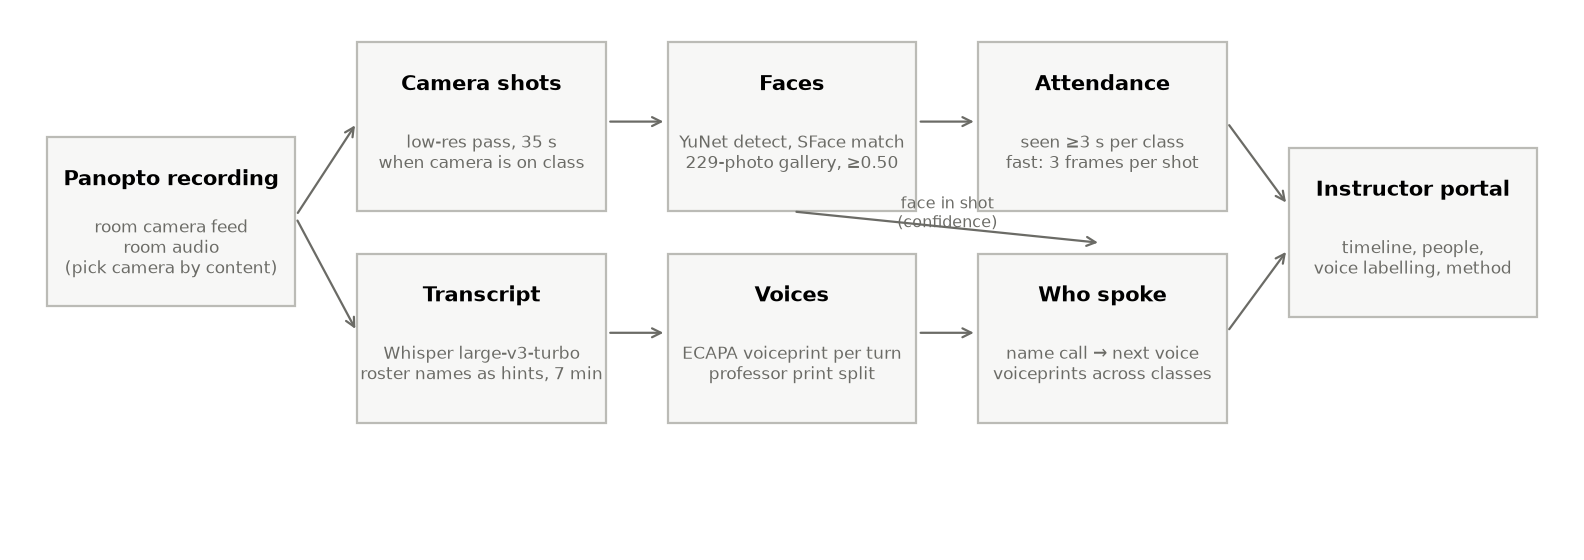
\includegraphics[width=\figw]{figures/f01_pipeline.png}
\caption{Pipeline. Everything runs after class; results appear in a local instructor portal.}\label{fig:pipeline}
\end{figure}

\section{Related work}
Automated attendance by face recognition has been demonstrated in controlled settings with frontal, close-range cameras; classroom deployments report sharp losses with distance, pose and occlusion. We use lightweight, permissively licensed models, YuNet for detection \cite{yunet} and SFace for recognition \cite{sface}, and measure them on a production PTZ camera rather than a purpose-mounted one. For speech we use Whisper \cite{whisper} and ECAPA-TDNN speaker embeddings \cite{ecapa,speechbrain}. Audio-visual active-speaker detection (e.g.\ TalkNet \cite{talknet}) reaches high accuracy on close faces but degrades for faces under 64\,px, which is where our classroom sits. Discourse-level measures of teaching, such as conversational uptake \cite{uptake}, motivate the transcript analyses. Emotion recognition in education is prohibited in the EU \cite{aiact}; we neither attempt nor recommend it.

\section{Setting and data}
\paragraph{Course and room.} One section (58 students) of a first-year MBA core course on leading people, taught by one instructor in a tiered classroom, observed in five sessions between 22 September and 8 October 2026 (each $\approx$120\,min of recording). Sessions mix lecture, cold-called case discussion, a quiz game and breaks. Table~\sessiontable\ref{tab:sessions} summarises them.

\paragraph{Recordings.} Each Panopto session holds a slides feed and a room-camera feed with room audio. The camera moves between presets (front of room and several views of the student tiers, Fig.~\ref{fig:views}). One session was stored at 1920$\times$1080; four were stored at 1024$\times$576. The stream labelled as the camera was in fact the slides in four of five sessions (Fig.~\ref{fig:swap}).

\paragraph{Reference faces.} 230 seating-chart headshots across all four sections of the course (229 usable). Matching against every section is what makes errors countable: a face named as a student of another section is certainly wrong.

\paragraph{Ground truth.} Section membership; desk name cards; names the instructor said aloud; a model reading the transcript in context; two independent model scoring passes. There was no attendance register, which is the main gap.

\begin{figure*}[t]\centering
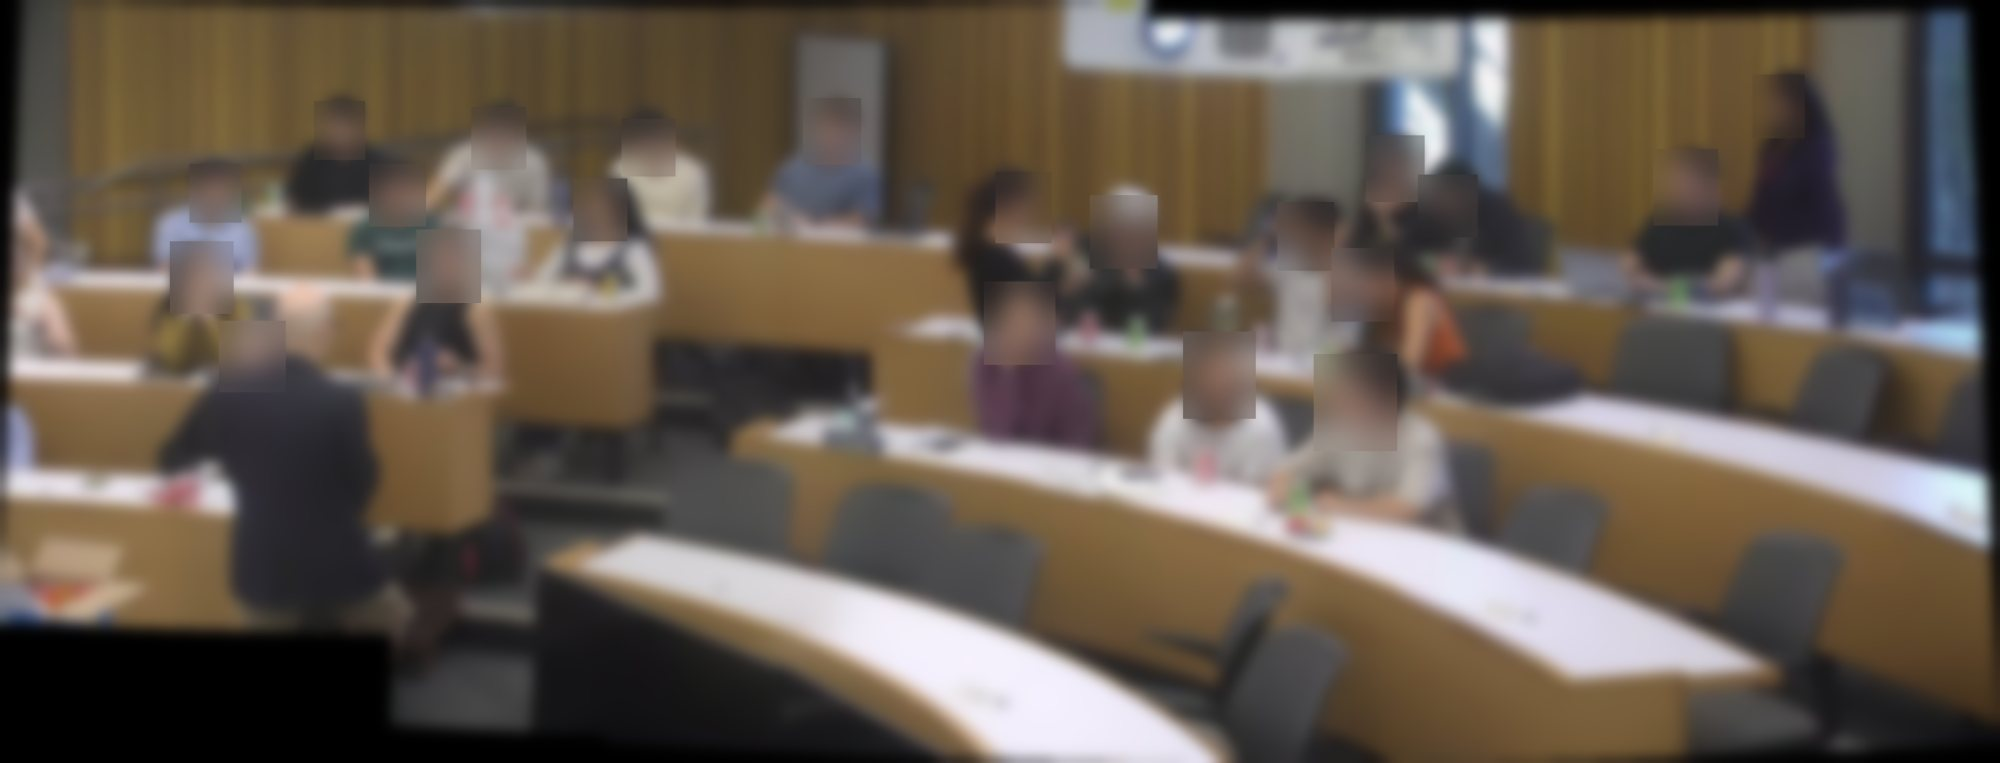
\includegraphics[width=\textwidth]{figures-redacted/panorama.jpg}
\caption{Part of the classroom, stitched from three overlapping camera presets on 8 October. Only presets that overlap cleanly can be joined; the rest are shown in Fig.~\ref{fig:views}.}\label{fig:pano}
\end{figure*}

\section{Method}
\subsection{Video}
A low-resolution pass (160$\times$90 grey, 4\,fps) over the whole recording finds camera moves; stills between moves are shots, grouped into presets by appearance, and a shot with $\geq$3 faces is a student shot. Faces $\geq$24\,px are detected with YuNet and embedded with SFace (128-d). A face is named when its best cosine similarity to the gallery is $\geq\tau{=}0.50$ and exceeds the runner-up by $\geq$0.05 (Fig.~\ref{fig:howfaces}). Faces are followed through a shot by box overlap; a student is \emph{present} in a class when named for $\geq$3\,s. Figure~\ref{fig:howshots} shows how shots are found and which frames the one-minute attendance pass reads.

\begin{figure*}[t]\centering
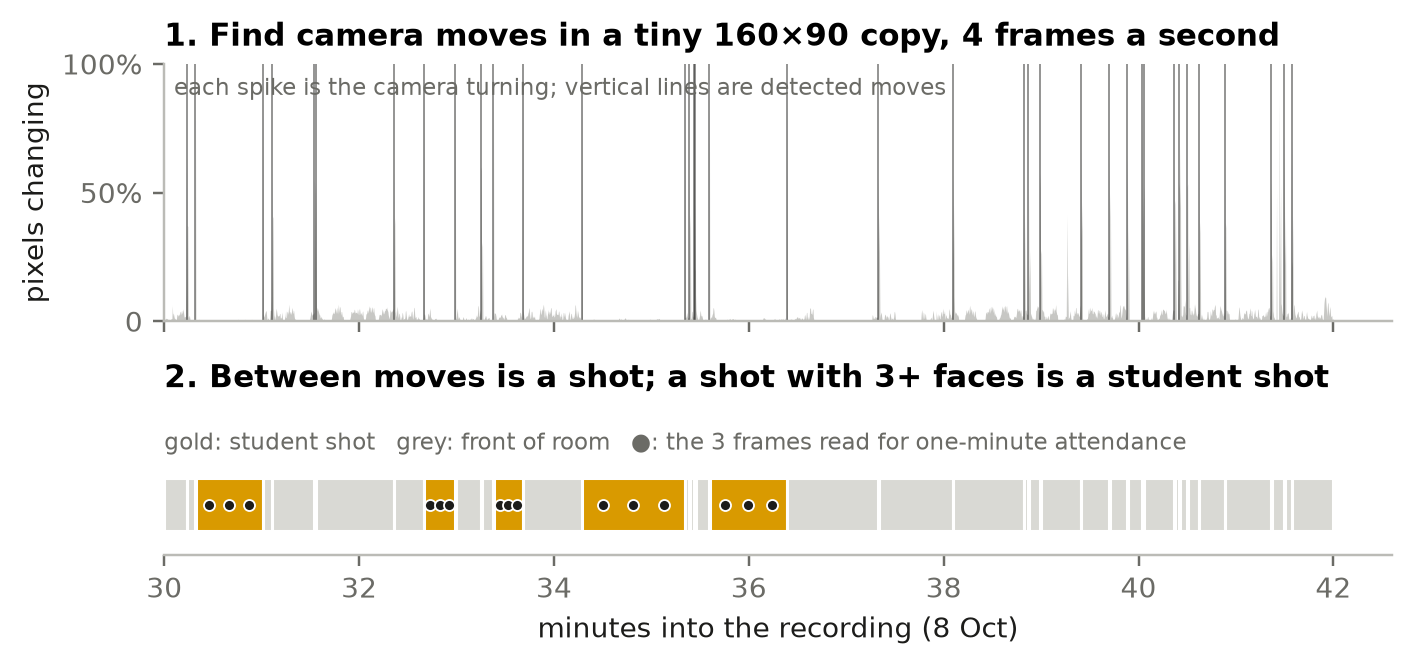
\includegraphics[width=0.9\textwidth]{figures/e01_how_shots.png}
\caption{How camera shots are found (twelve minutes of 8 October). The share of pixels changing between frames spikes when the camera turns; the stills between turns are shots. Student shots (gold) are where faces are read; the one-minute pass reads only the three marked frames in each.}\label{fig:howshots}
\end{figure*}

\begin{figure}[t]\centering
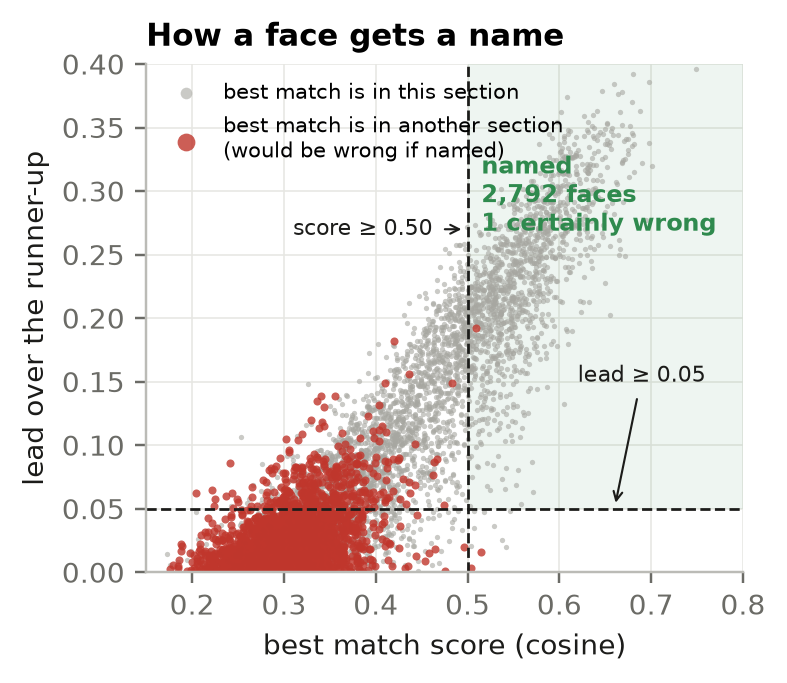
\includegraphics[width=0.95\figw]{figures/e02_how_faces.png}
\caption{How a face gets a name, for every face detected at 1080p on 8 October (grey points subsampled). A face is named only in the shaded corner: score $\geq$0.50 and a lead of $\geq$0.05 over the next-best student. Red faces' best match is a student from another section, so naming them would certainly be wrong; the rule rejects all but one. Table~\ref{tab:id} uses a 2-second sample of the same class.}\label{fig:howfaces}
\end{figure}

\subsection{Audio}
Audio is transcribed with Whisper large-v3-turbo (mlx on Apple Silicon) with the section's first names and course terms as prompt. Words form turns at pauses of 0.8\,s; each turn of $\geq$1.5\,s gets an ECAPA voiceprint. The instructor print is the largest voice cluster of one session; it transfers across sessions (cosine 0.96--0.97).

\subsection{Naming voices}
When the instructor ends a sentence with a student's first name (``\ldots[name], go.'') and a non-instructor turn of $\geq$5\,s starts within 20\,s, that turn is labelled with the student. Labelled turns form the student's voiceprint; other student turns in any class are named when they match a print at $\geq$0.50 with a 0.05 margin. A portal lets a person label unknown voice clusters, which become anchors. Figure~\ref{fig:howvoices} follows one student through the five classes.

\begin{figure*}[t]\centering
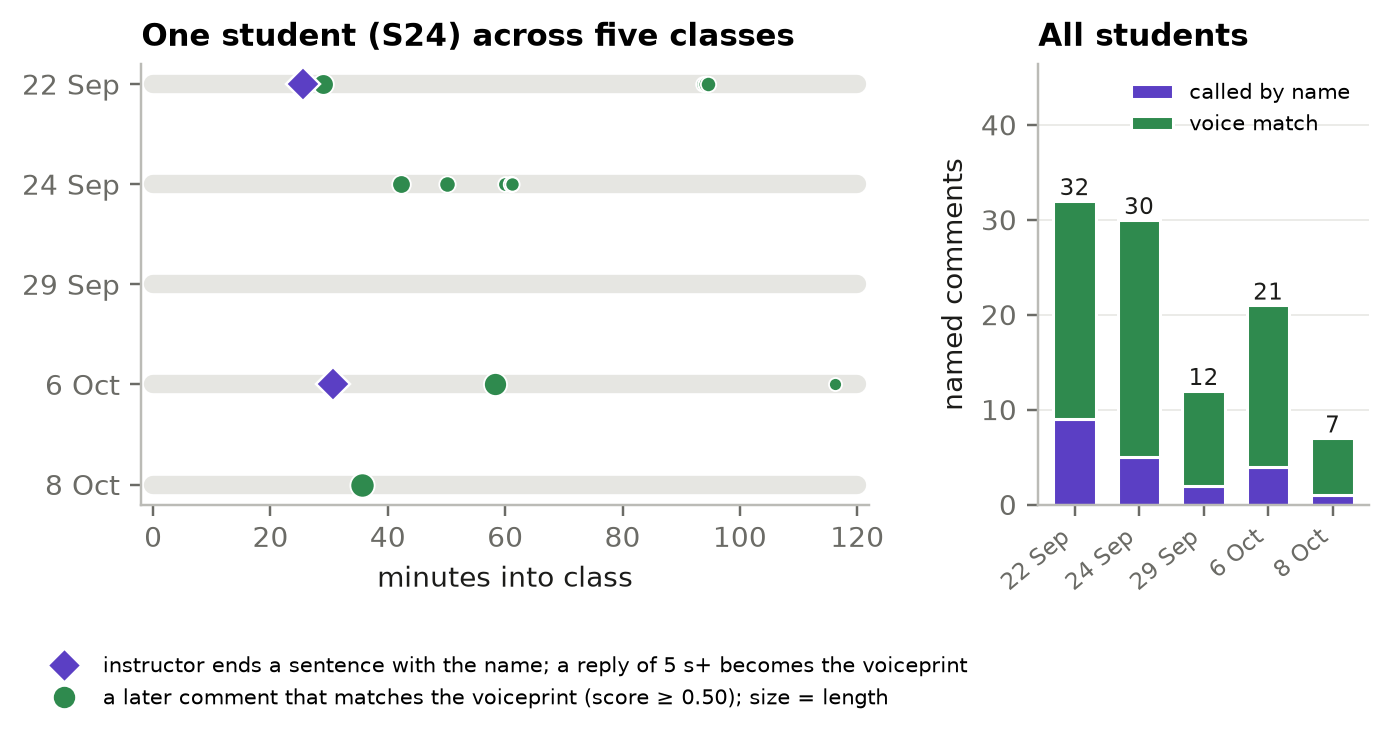
\includegraphics[width=0.9\textwidth]{figures/e03_how_voices.png}
\caption{How a voice gets a name. Left: one student, anonymised. Two name calls (diamonds) gave the voiceprint; every other comment (circles) was matched to it by voice, including in classes where the student was never called on. Right: named comments per class for all students, by method.}\label{fig:howvoices}
\end{figure*}

\subsection{Evaluation without hand labels}
Identification errors are certain cross-section matches, scaled by 229/172 to estimate within-section errors. Verification uses same-seat pairs one second apart (same person) and same-frame pairs (different people). Voice accuracy is leave-one-out over name-call-labelled turns, within and across classes.

\section{Results}
\subsection{Naming a visible face is precise}
Table~\idtable\ref{tab:id} and Fig.~\ref{fig:id} show the identification trade-off on the 1080p session. At $\tau{=}0.50$, 1{,}393 faces were named with no certain error (estimated error below $\approx$0.3\%, 95\% confidence); at 0.40 there were 19. The same seat a second later received the same name in 744 of 744 cases. Verification on the room's own footage (Table~\vertable\ref{tab:ver}, Fig.~\ref{fig:ver}) shows why the library default of 0.363 is unsafe for a full class: an unknown face would clear the bar against at least one of 70 students 44\% of the time, against 0.7\% at 0.50.

\begin{figure}[t]\centering
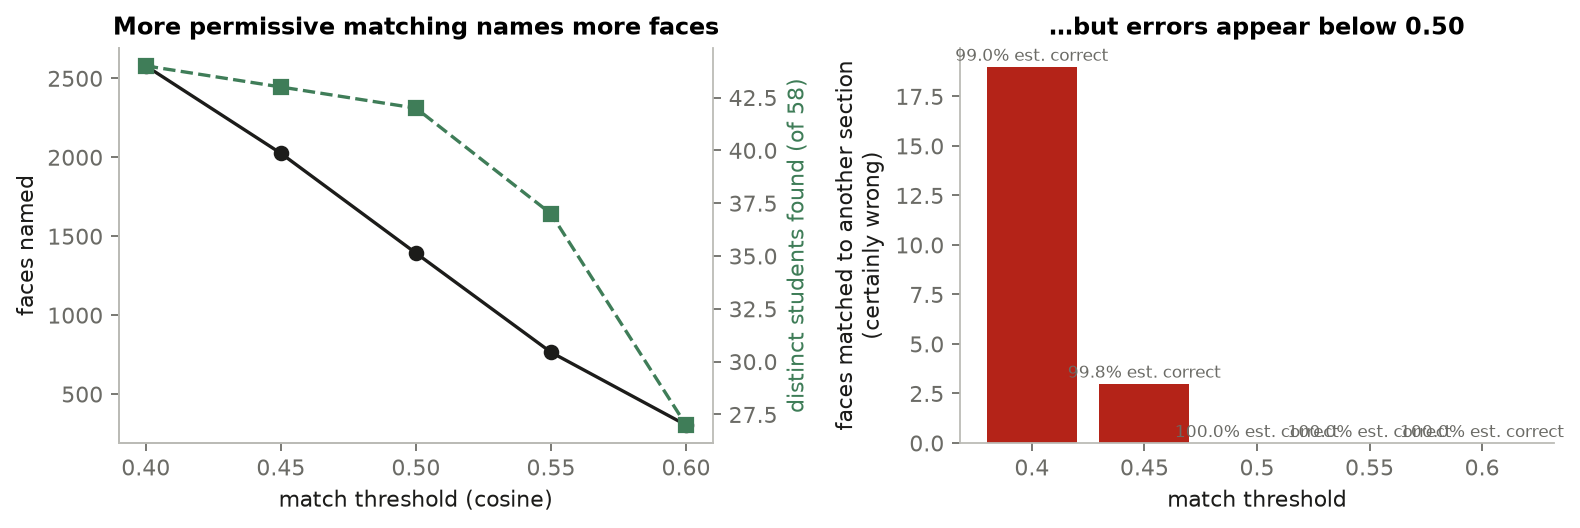
\includegraphics[width=\figw]{figures/f02_identification_thresholds.png}
\caption{Faces named, students found and certain errors by threshold (1080p).}\label{fig:id}
\end{figure}
\begin{figure}[t]\centering
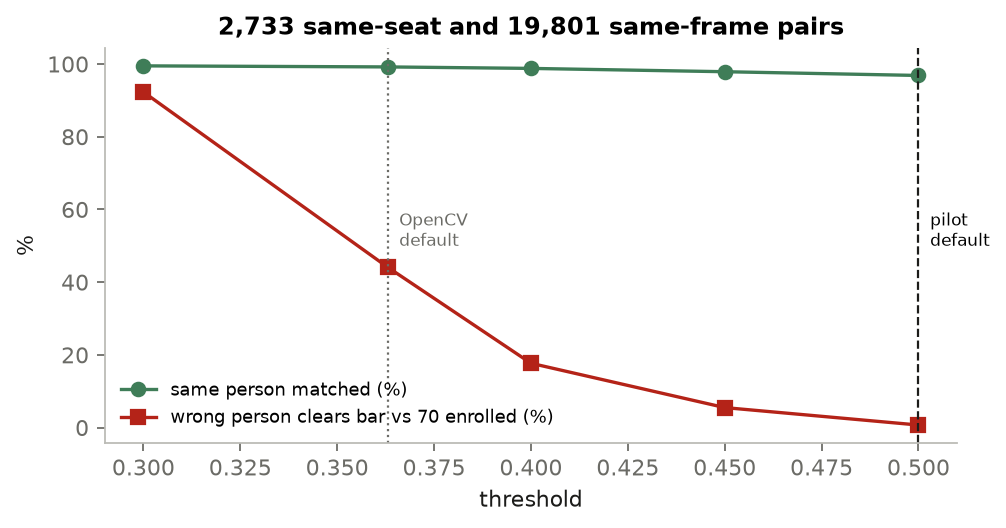
\includegraphics[width=0.92\figw]{figures/f03_verification.png}
\caption{Same-person match rate and false-match rate against a 70-person gallery.}\label{fig:ver}
\end{figure}

Figures~\ref{fig:tag8} and \ref{fig:tag22} show every detected face in the busiest student shot of two classes with its best match score (faces blurred in this edition). In Fig.~\ref{fig:tag8}, one face named at 0.51 sits directly above a desk card with the same name, an independent confirmation. Amber faces scored below the threshold or margin and stay unnamed.

\begin{figure*}[p]\centering
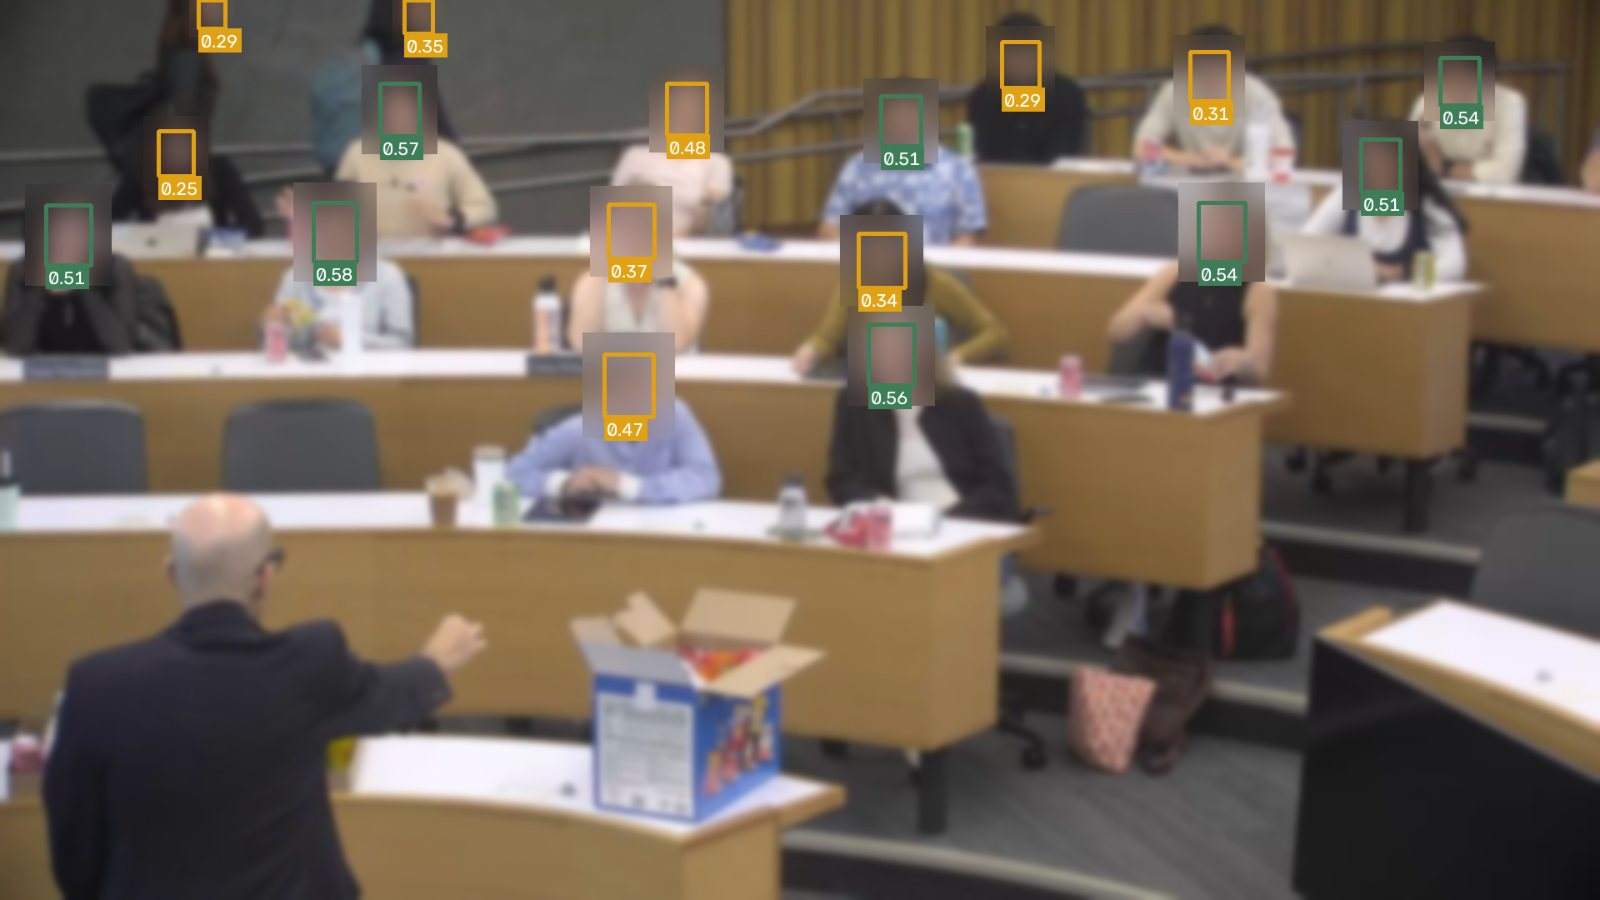
\includegraphics[width=\textwidth]{figures-redacted/tagged_2026-10-08.jpg}
\caption{Busiest student shot, 8 October (1920$\times$1080). Green: named at $\geq$0.50 with margin. Amber: best score, left unnamed. Faces blurred.}\label{fig:tag8}
\vspace{0.8em}
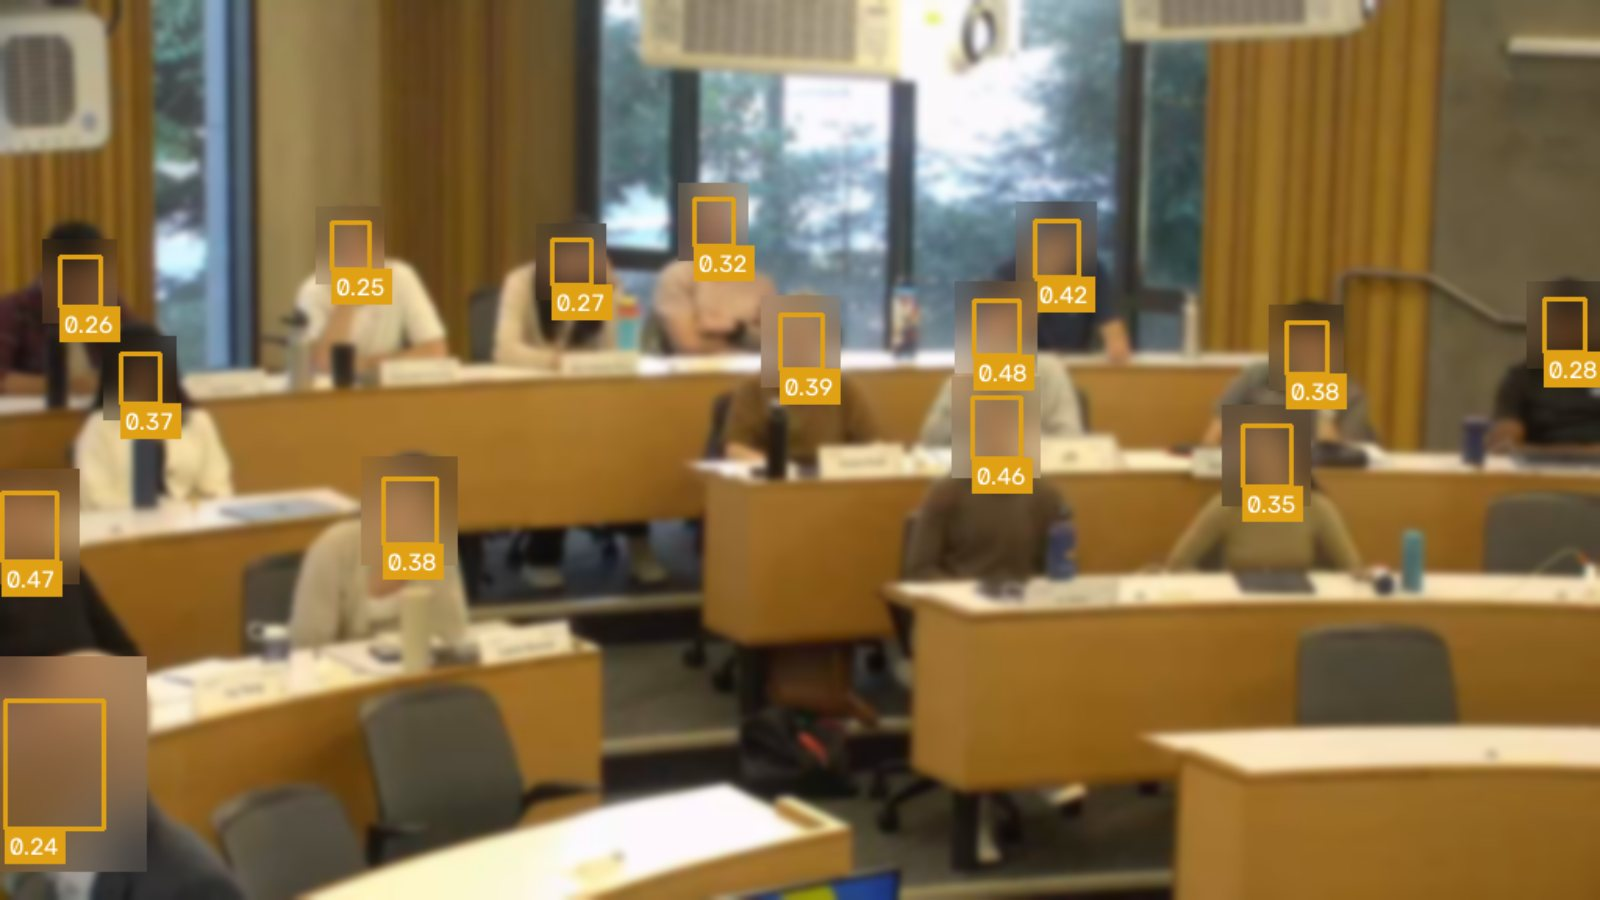
\includegraphics[width=\textwidth]{figures-redacted/tagged_2026-09-22.jpg}
\caption{Busiest student shot, 22 September (1024$\times$576). Faces are about half the size; scores fall and more faces are left unnamed. Faces blurred.}\label{fig:tag22}
\end{figure*}

\paragraph{Name cards.} On-device text recognition on zoomed tiles read 309 desk cards in 298 student shots; every reading was a real section name. Only 5 of 58 students had a card the camera could read, and the card agreed with the face above it in 15 of 22 links; all 7 disagreements were one card linked to the adjacent student.

\subsection{Camera coverage limits attendance}
The camera serves remote viewers: it follows the instructor and the active microphone. Student shots covered 22--33\% of discussion classes and 11\% of the quiz-game class (Fig.~\ref{fig:cov}). Per class the system named 33--42 of 58 students for $\geq$3\,s (Fig.~\ref{fig:att}); with that rule, certain errors across all five classes fell from 10 to 3. Counting faces seen but not named by clustering was unstable (11--28 people depending on settings), so absence cannot be inferred. Across classes coverage accumulates: 55 of 58 were recognised at least once and 31 in four or five classes (Table~\ref{tab:students}, Fig.~\ref{fig:attname}).

\begin{figure*}[t]\centering
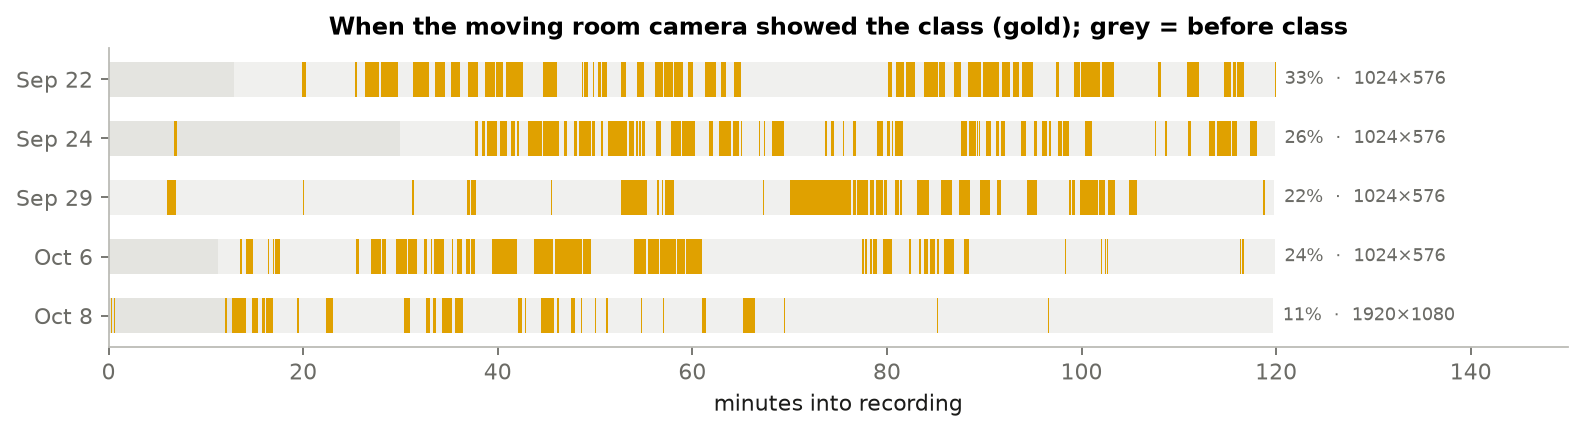
\includegraphics[width=\textwidth]{figures/f04_camera_coverage.png}
\caption{When the room camera showed the class (gold). Grey: before class (music, empty room).}\label{fig:cov}
\end{figure*}
\begin{figure}[t]\centering
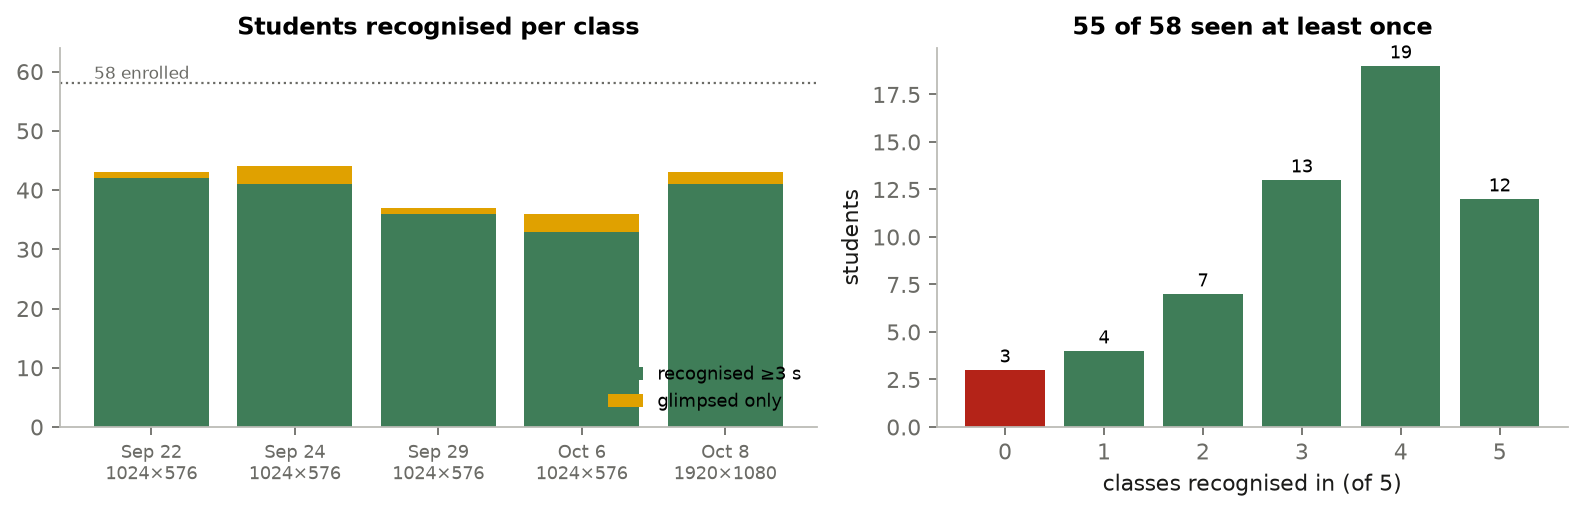
\includegraphics[width=\figw]{figures/f05_attendance.png}
\caption{Left: recognised per class. Right: students by number of classes recognised.}\label{fig:att}
\end{figure}

\subsection{Attendance in a minute}
Reading three frames from each student shot (135--165 frames rather than 7{,}200) found 86--88\% of the students a full scan finds, with no certain errors at 1080p, in 57--65\,s end to end; most of that is the shot-finding pass (Fig.~\ref{fig:fast}).
\begin{figure}[t]\centering
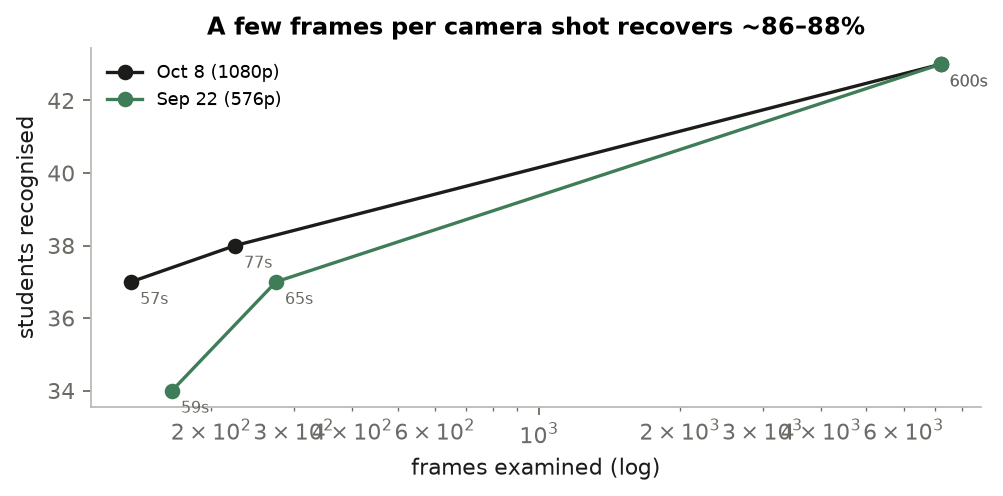
\includegraphics[width=0.92\figw]{figures/f08_fast_attendance.png}
\caption{Students recognised versus frames examined.}\label{fig:fast}
\end{figure}

\subsection{Speech}
Instructor speech was $\approx$95\% clean; student points were recoverable in most turns. With the class list as a prompt, recognisable called names rose from 4 to 9--10 of 10, and 13--22 section first names appeared per class. Large-v3-turbo on the laptop GPU transcribed two hours in 6.5--7.2\,min (Fig.~\ref{fig:asr}). Pause-split turns blur speakers: 12 of 32 turns the voice split called ``student'' were the instructor, music or the quiz scorekeeper, and about 10 instructor turns contained student speech. Scanning 2\,s windows against the instructor print recovered 7 of 10 hidden student segments with 2 false alarms in 40 instructor turns.
\begin{figure}[t]\centering
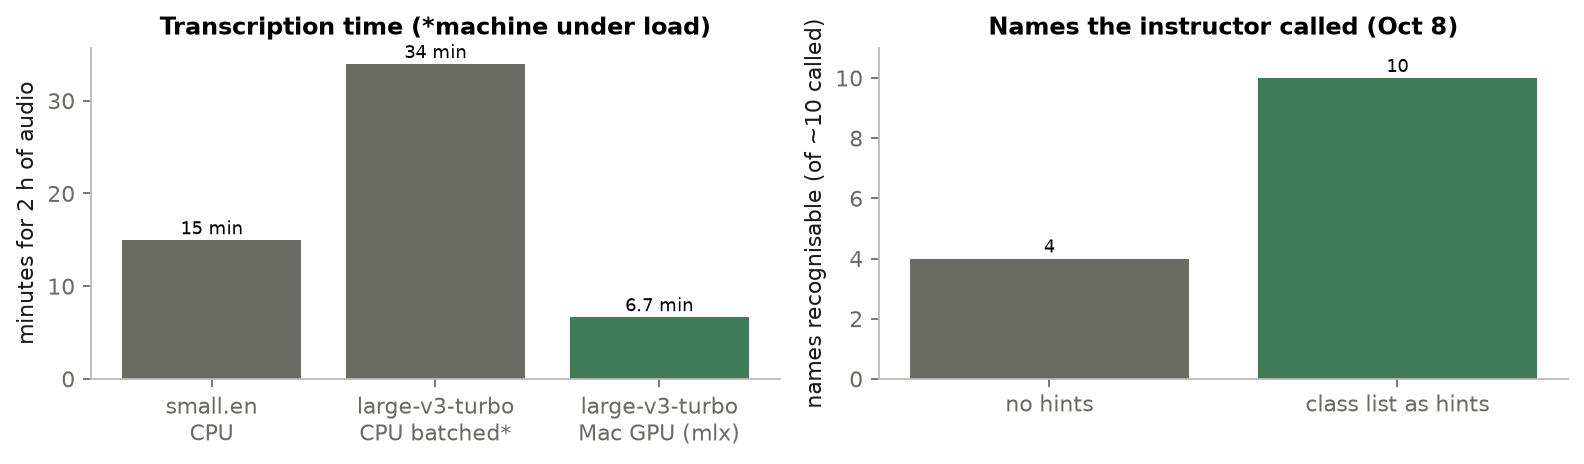
\includegraphics[width=\figw]{figures/f11_transcription.png}
\caption{Transcription time and recognisable called names.}\label{fig:asr}
\end{figure}

\subsection{Identifying the speaker}
The camera follows the microphone: all 15 genuine student comments in one class had the camera on students during or just before them, and a student shot began within 16\,s of a comment three times more often than chance. The speaker was in shot for 8 of 9 known comments, but among a median of 16 faces (9 named), gaze of others picked the speaker 0 times, mouth motion once, nearest-centre 0 and largest face 0 (Fig.~\ref{fig:cues}).

\begin{figure}[t]\centering
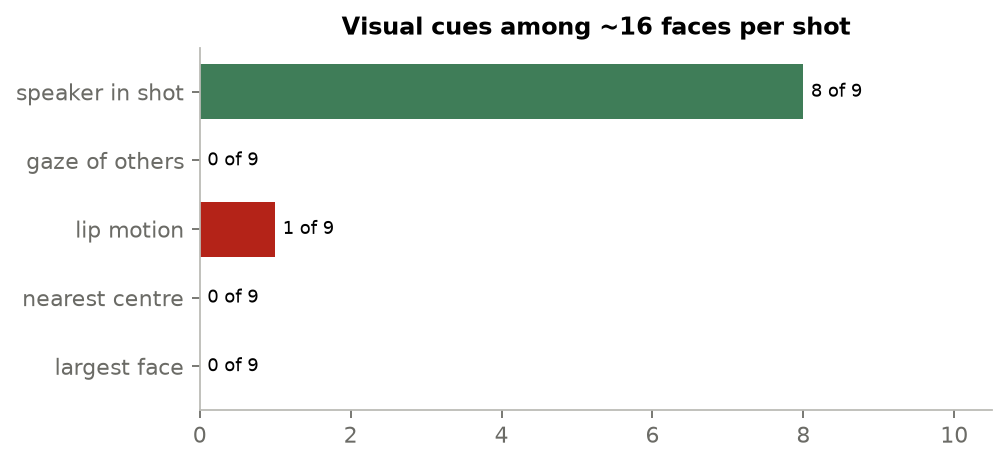
\includegraphics[width=0.92\figw]{figures/f10_speaker_cues.png}
\caption{Visual cues against known speakers.}\label{fig:cues}
\end{figure}

Voices separate well. Within a class, voiceprints matched 11 of 11 held-out comments (same-speaker median similarity 0.78, different-speaker 0.13). Across classes, labels from any name mention got 4 of 10; requiring the name to end the instructor's sentence and a reply of $\geq$5\,s got 6 of 6 (Fig.~\ref{fig:voice}). The single same-student pair at 0.07 exposed a mislabelled anchor, which is how errors in this method surface. After five classes, 16 students have voiceprints (Table~\voicetable\ref{tab:voices}) and 102 comments are named (81 by voice match), yet only 6--22\% of student-side audio per class. Sixteen voice matches come from a class in which the camera never recognised that student; the portal flags them.

\begin{figure}[t]\centering
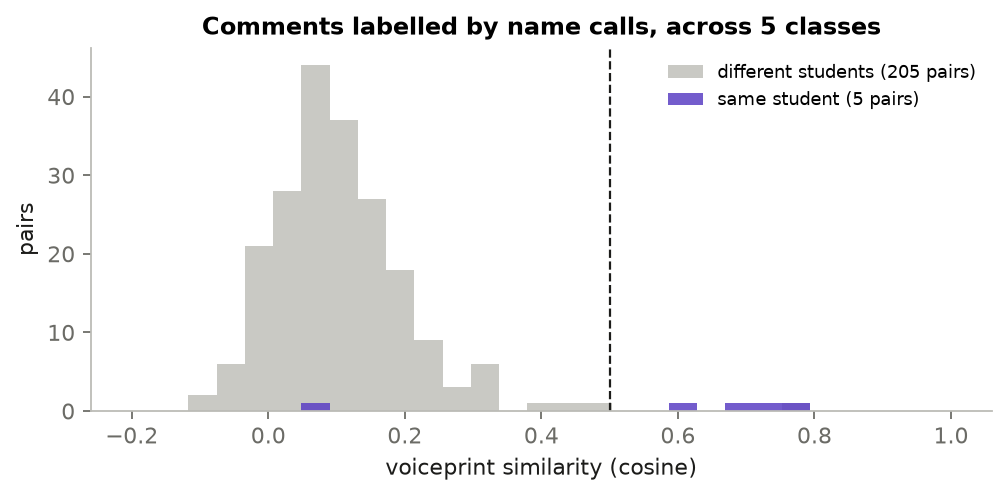
\includegraphics[width=0.92\figw]{figures/f09_voice_similarity.png}
\caption{Pairwise voiceprint similarity of name-call-labelled comments.}\label{fig:voice}
\end{figure}

\begin{figure*}[t]\centering
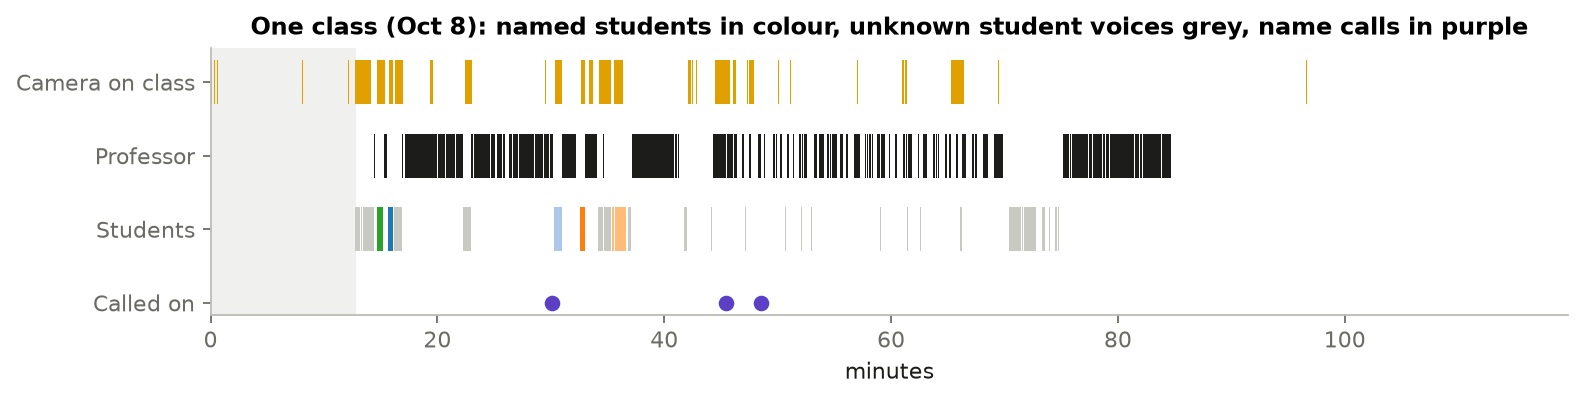
\includegraphics[width=\textwidth]{figures/f07_class_timeline.png}
\caption{One class on a timeline (8 October): camera on students, instructor speech, student speech (named in colour, unknown in grey) and name calls.}\label{fig:timeline}
\end{figure*}

\subsection{Scoring contributions}
Two independent Claude passes scored each student turn of one class on four 1--5 criteria (relevance, evidence, building on others, insight). Scores were identical in 124 of 128 cases and never differed by more than one point (Fig.~\ref{fig:rubric}); both passes flagged the same 12 turns as non-student audio. No instructor has yet scored a blind sample, so validity is untested. From the transcript alone the model also produced a class-phase timeline, a discussion summary, the questions students asked, an exam review sheet with all 20 quiz questions and follow-up email points.
\begin{figure}[t]\centering
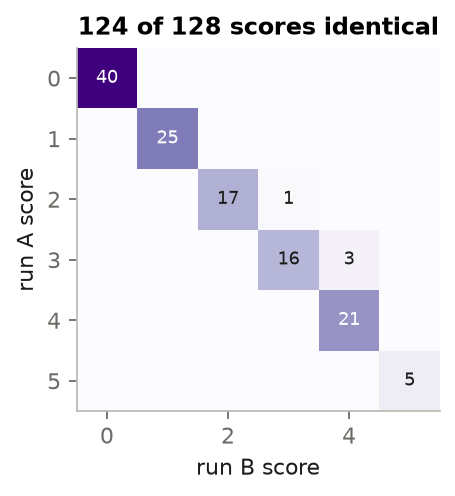
\includegraphics[width=0.72\figw]{figures/f12_rubric_agreement.png}
\caption{Agreement between two scoring passes.}\label{fig:rubric}
\end{figure}

\subsection{Speed and cost}
Per two-hour class on one laptop: download $\approx$1\,min, shot finding 35\,s, fast attendance $\approx$1\,min, transcript $\approx$7\,min, voiceprints $\approx$1\,min (Fig.~\ref{fig:time}). On a cloud GPU we estimate $\approx$\$0.10 per class.
\begin{figure}[t]\centering
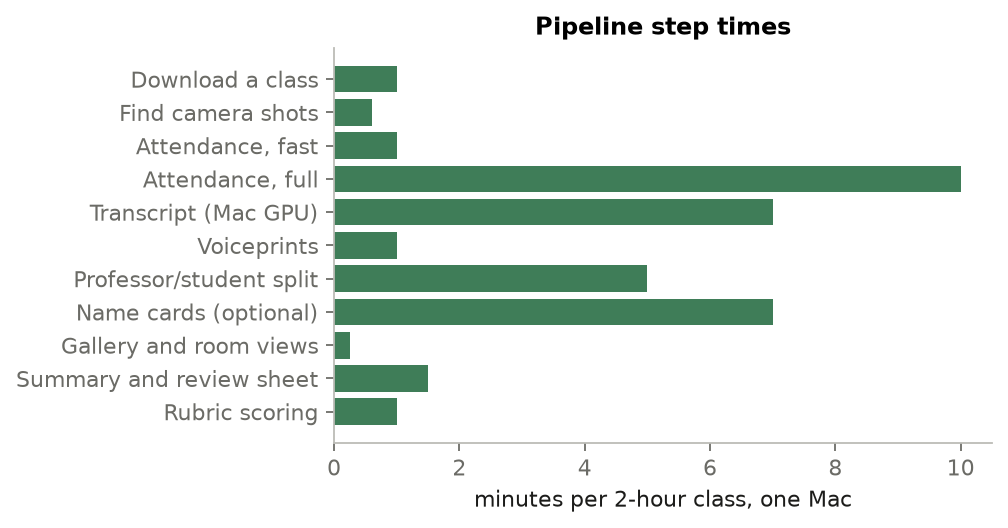
\includegraphics[width=0.92\figw]{figures/f13_timings.png}
\caption{Step times per class on one Mac.}\label{fig:time}
\end{figure}

\section{Discussion}
\paragraph{What worked.} Naming a visible face; term-level presence; one-minute attendance; transcripts with names; naming a voice after a name call and carrying it across classes; transcript summaries and review sheets.
\paragraph{What partly worked.} Absence (coverage-limited); naming most student talk (6--22\% after five classes); instructor/student separation at turn boundaries; contribution scores (consistent, unvalidated).
\paragraph{What failed.} Picking the speaker from video at 30--60\,px; late arrival and early exit; name cards as an attendance source.

\paragraph{Data-quality traps.} (1) Feed labels swap between sessions (Fig.~\ref{fig:swap}); identify the camera by content. (2) Resolution varies (1080p vs 576p) and halves face size; keep originals. (3) Recordings start early (once by 30\,min) and include music, which transcribes as student speech. (4) Guests and the quiz scorekeeper look like students until labelled. (5) The PTZ camera is aimed for remote viewers, so it films quiet students least.

\begin{figure}[t]\centering
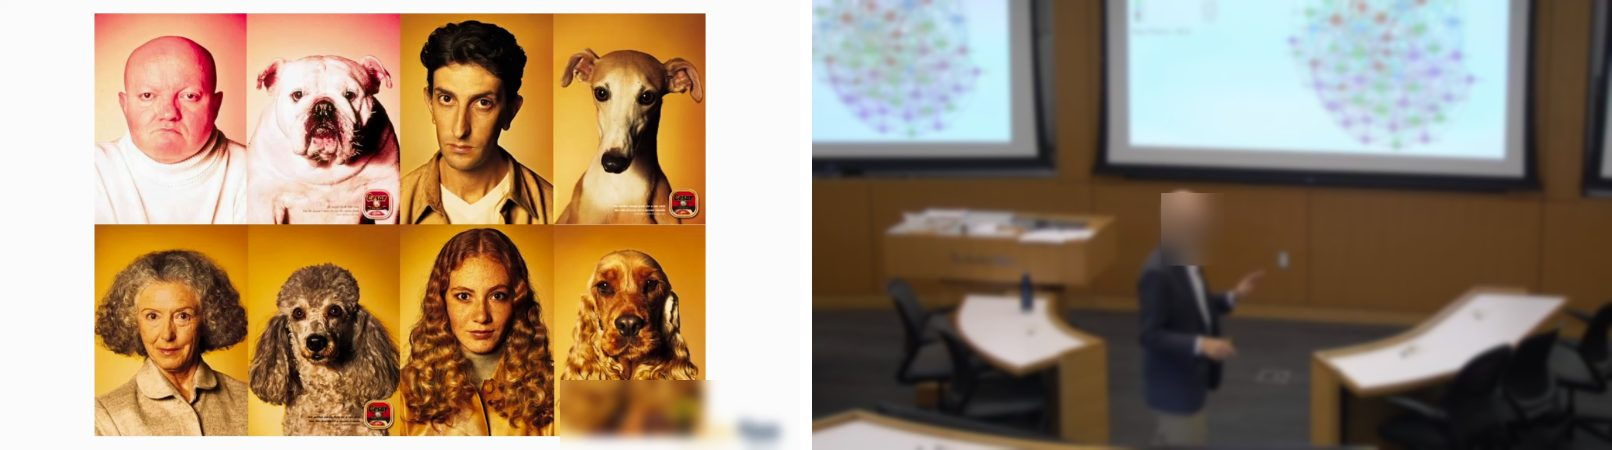
\includegraphics[width=\figw]{figures-redacted/feed_swap.jpg}
\caption{29 September: the stream Panopto labelled as the room camera (left) is the slides; the other stream (right) is the camera.}\label{fig:swap}
\end{figure}

\section{Limitations}
One section, one room, one instructor, five sessions. No attendance register, so attendance recall is unmeasured. Voice results rest on 8--16 speakers and a handful of held-out comments. Error estimates assume errors spread evenly across the gallery. Contribution scores are not validated against the instructor, and we did not test for differences in error by accent, gender or skin tone, which must precede any use affecting students.

\section{What it would take}
A teaching assistant's tick sheet for three to five classes (true recall); the room controller's log of which desk microphone was pressed (speaker seat, likely free); keeping original-resolution camera files; a fixed wide camera on the student tiers (\$1.4--4.3k per room); a ceiling microphone array with talker position if no microphone log exists (\$4--7.6k); Panopto administrative API access; an instructor's blind scores on 20--30 comments; and P4-approved storage with a GPU host ($\approx$\$0.10 per class).

\section{Ethics and data handling}
Students consented to face recognition, voiceprints and recording, and the administration approved this research use. Face templates are P4 data under UC Berkeley's classification and per-student records are FERPA education records. Recordings, templates and voiceprints remain on the pilot machine; recordings, face templates, voiceprints and the identified results stay on the pilot machine. This public edition replaces student names with anonymous ids and blurs student faces; the companion portal uses pseudonyms and has no audio or transcript text. Publication beyond the institution should pass human-subjects review. We did not infer emotion or attention, rank students publicly or grade automatically.

\section{Conclusion}
Lecture capture that schools already run can tell an instructor who was in the room and what was said. Face naming was precise, transcripts were accurate once the model had the class list, and the instructor's habit of calling students by name was enough to learn their voices. The remaining gaps come from where the camera points and from not knowing which desk microphone was pressed. A microphone log, a fixed wide camera on the student tiers and a week of hand-taken attendance would close most of them.

{\small
\begin{thebibliography}{9}\setlength{\itemsep}{1pt}
\bibitem{yunet} W.~Wu, H.~Peng, S.~Yu. YuNet: A tiny millisecond-level face detector. \emph{Machine Intelligence Research}, 2023.
\bibitem{sface} Y.~Zhong, W.~Deng, et al. SFace: Sigmoid-constrained hypersphere loss for robust face recognition. \emph{IEEE TIP}, 2021.
\bibitem{whisper} A.~Radford et al. Robust speech recognition via large-scale weak supervision. \emph{ICML}, 2023.
\bibitem{ecapa} B.~Desplanques, J.~Thienpondt, K.~Demuynck. ECAPA-TDNN: Emphasized channel attention, propagation and aggregation in TDNN based speaker verification. \emph{Interspeech}, 2020.
\bibitem{speechbrain} M.~Ravanelli et al. SpeechBrain: A general-purpose speech toolkit. arXiv:2106.04624, 2021.
\bibitem{talknet} R.~Tao et al. Is someone speaking? Exploring long-term temporal features for audio-visual active speaker detection. \emph{ACM Multimedia}, 2021.
\bibitem{uptake} D.~Demszky et al. Measuring conversational uptake: A case study on student-teacher interactions. \emph{ACL}, 2021.
\bibitem{aiact} Regulation (EU) 2024/1689 (Artificial Intelligence Act), Art.~5(1)(f).
\bibitem{ucb} UC Berkeley Information Security Office. Data Classification Guideline (P1--P4).
\end{thebibliography}}

\onecolumn
\appendix
\section{Every camera view of the class (faces blurred)}
\begin{figure}[H]\centering
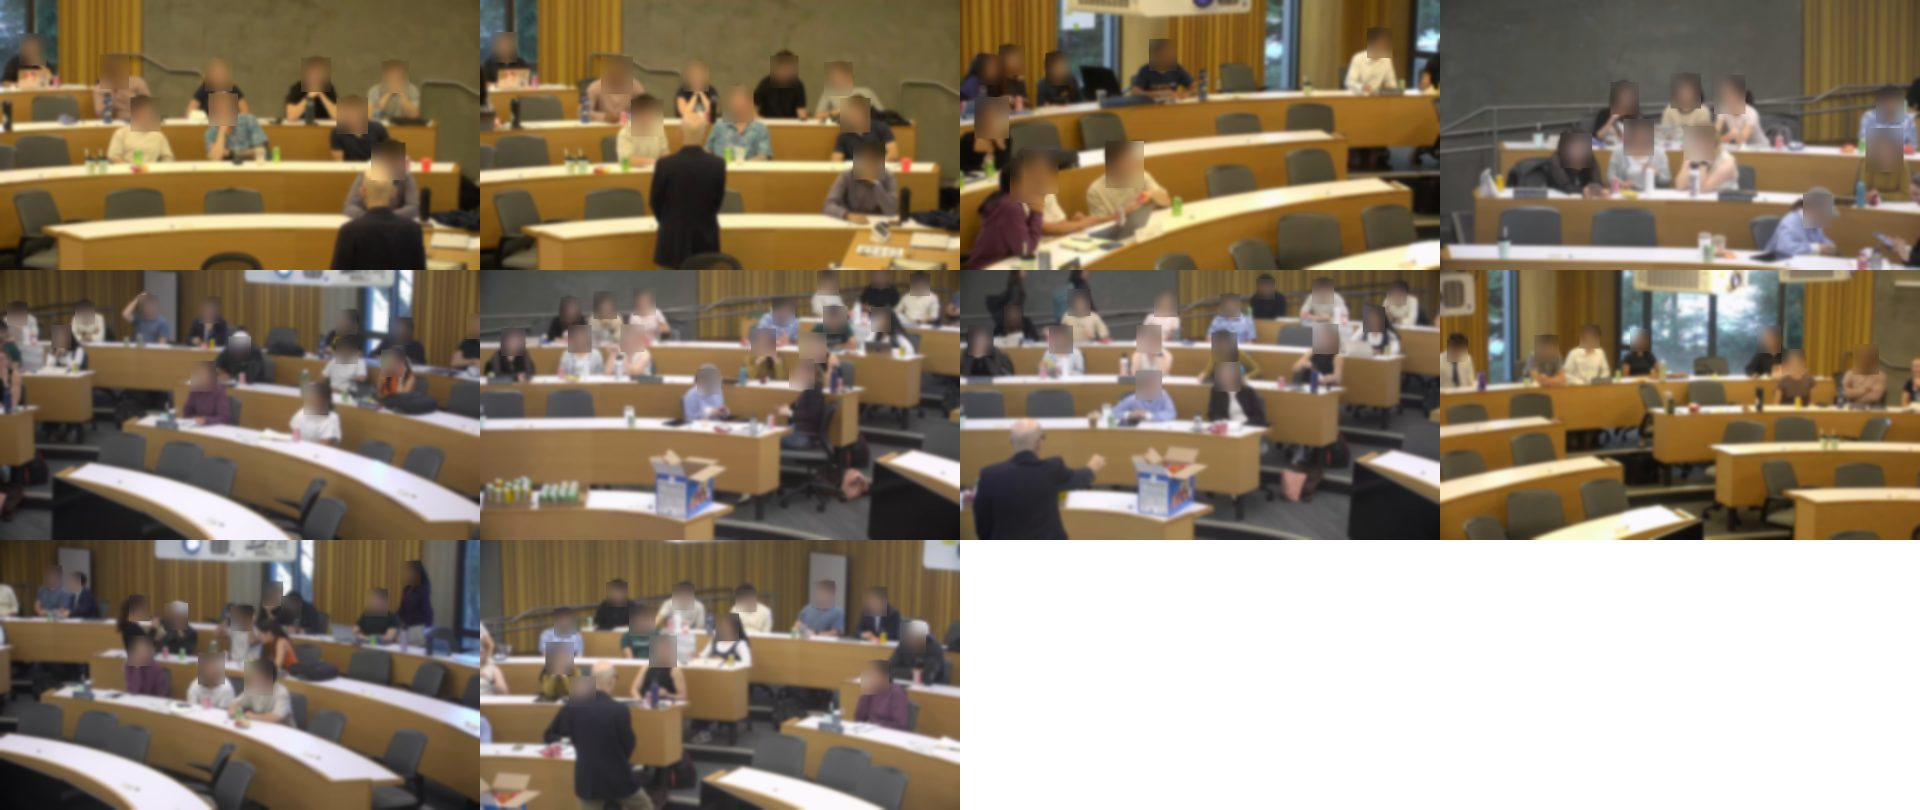
\includegraphics[width=0.85\textwidth]{figures-redacted/camera_views.jpg}
\caption{The clearest frame from each camera preset that showed students on 8 October.}\label{fig:views}
\end{figure}

\section{Student shots from the other classes (faces blurred)}
\begin{figure}[H]\centering
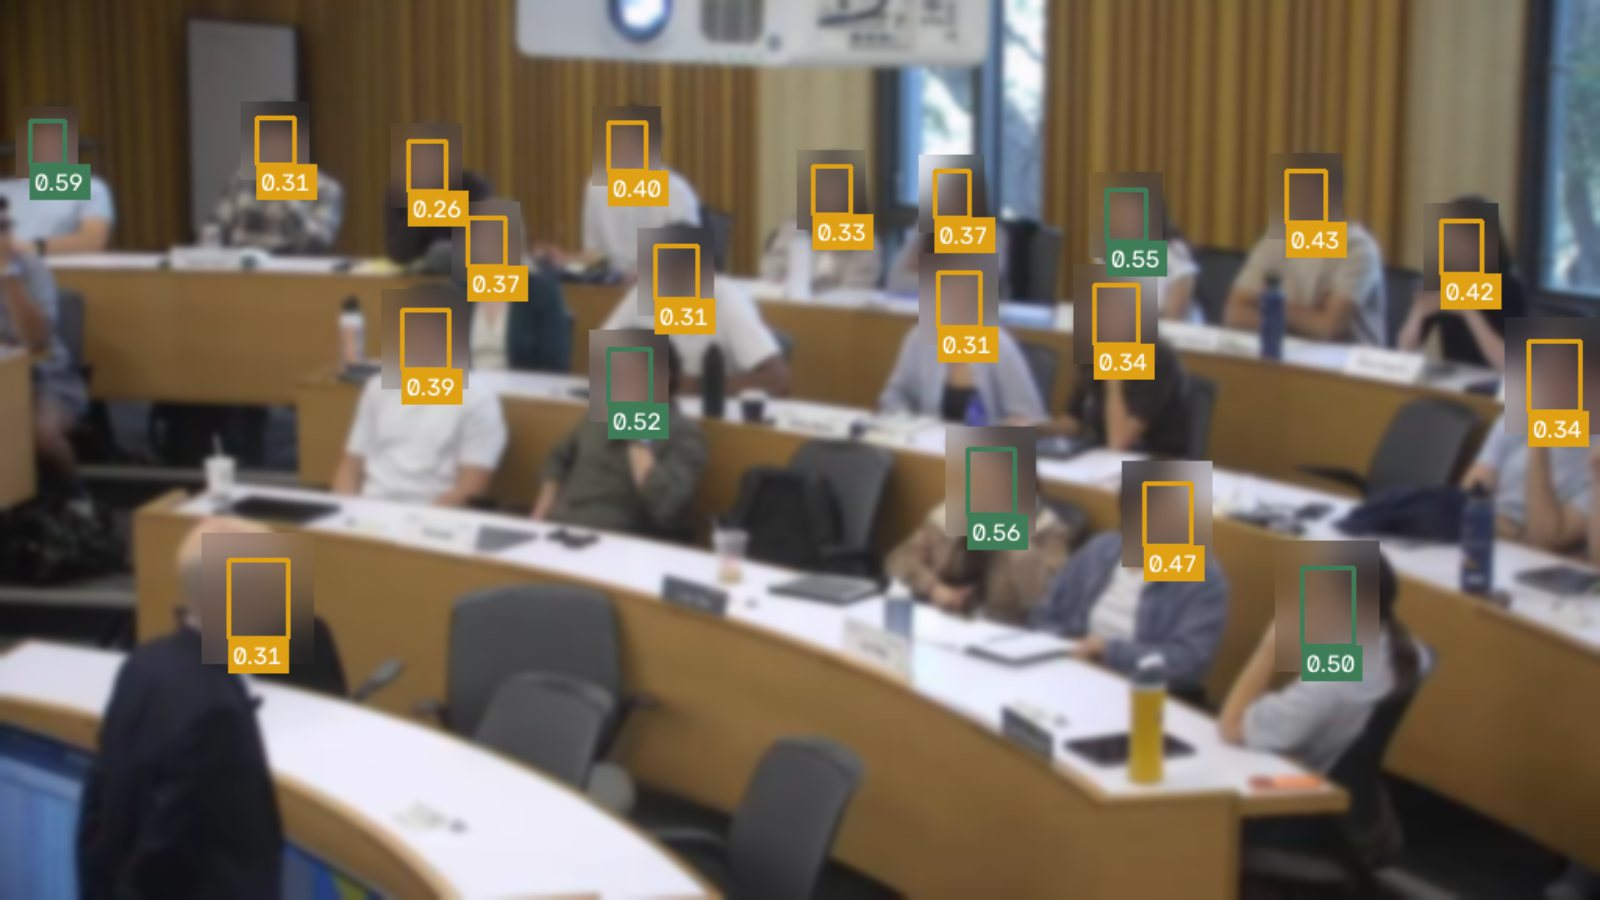
\includegraphics[width=0.49\textwidth]{figures-redacted/tagged_2026-09-24.jpg}\hfill
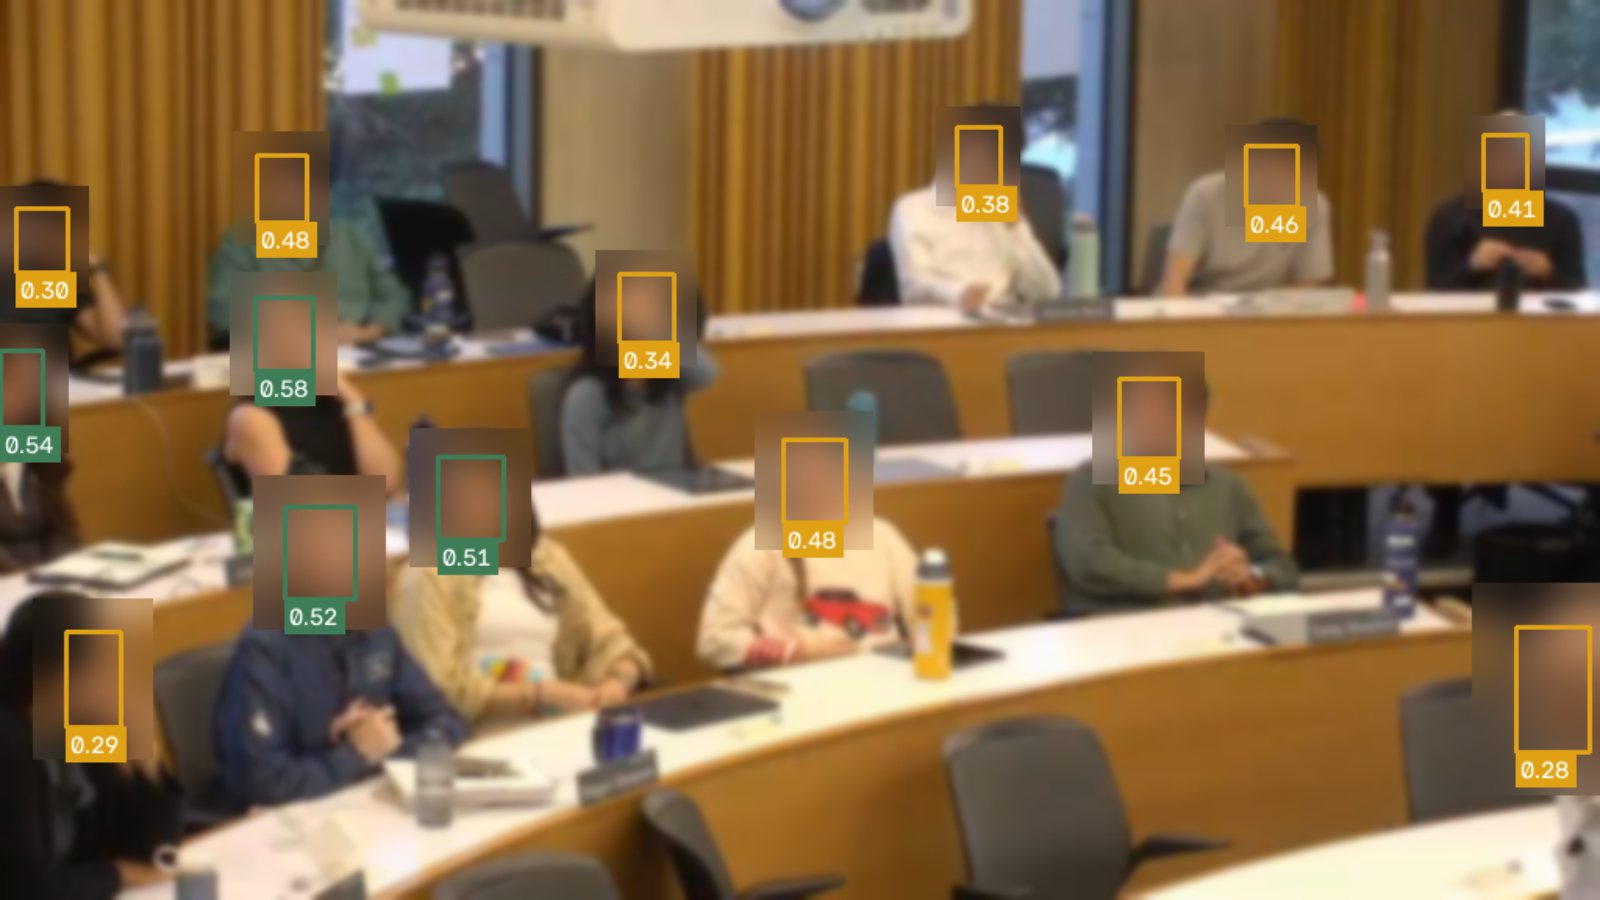
\includegraphics[width=0.49\textwidth]{figures-redacted/tagged_2026-09-29.jpg}\\[4pt]
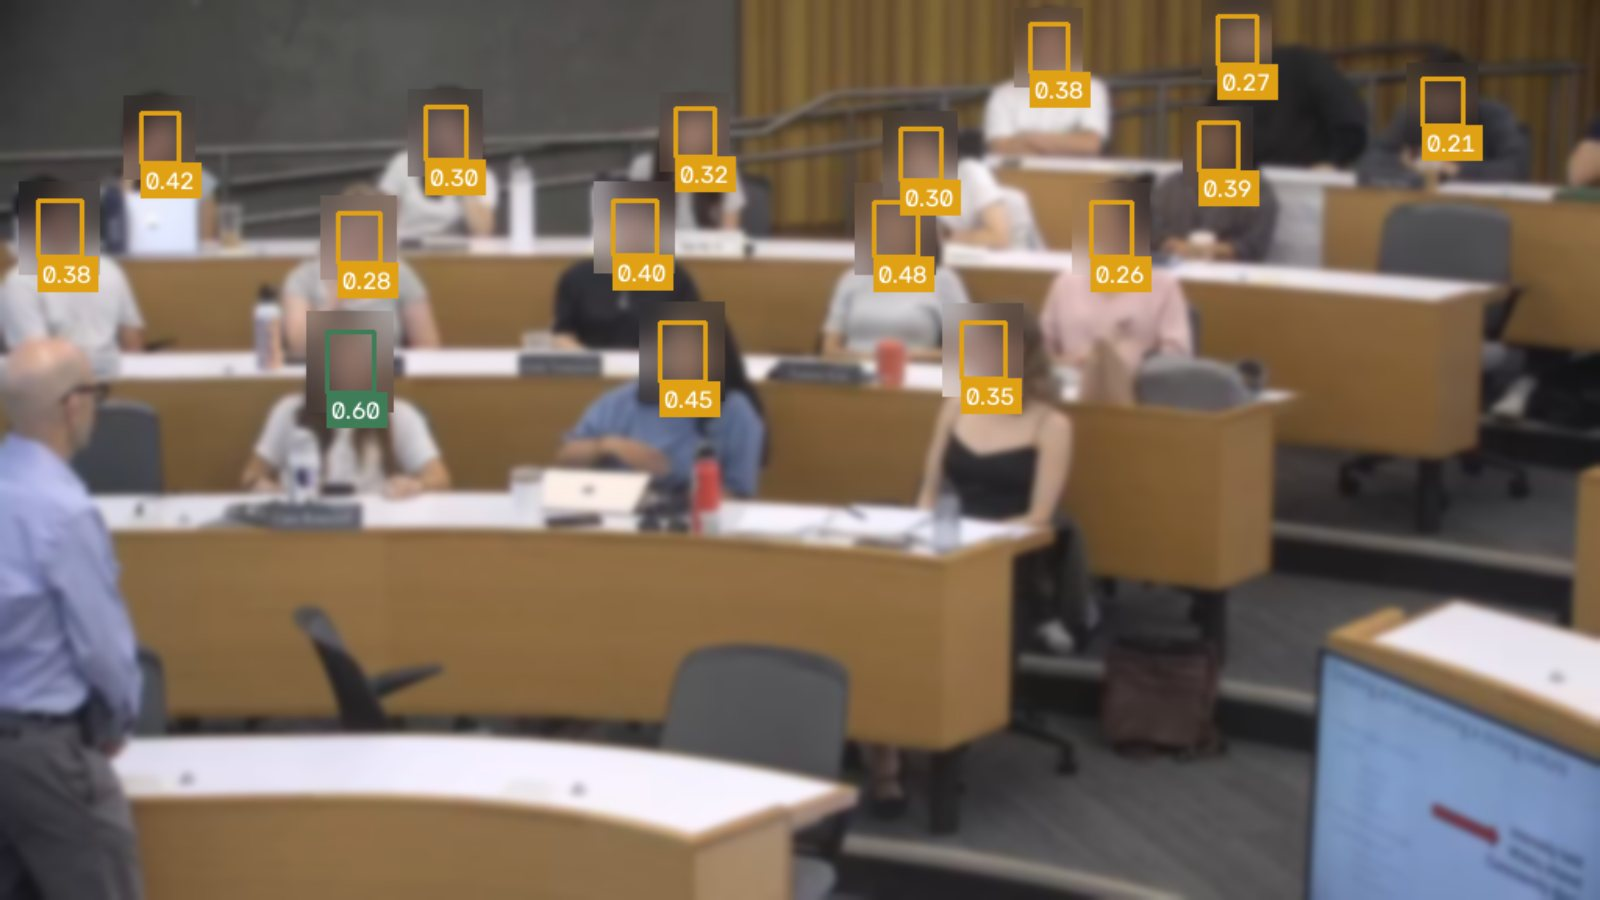
\includegraphics[width=0.49\textwidth]{figures-redacted/tagged_2026-10-06.jpg}
\caption{Busiest student shots on 24 September, 29 September and 6 October (all 1024$\times$576).}
\end{figure}

\clearpage
\section{Per-student results}
\studenttable

\clearpage
\section{Attendance by student}
\begin{figure}[H]\centering
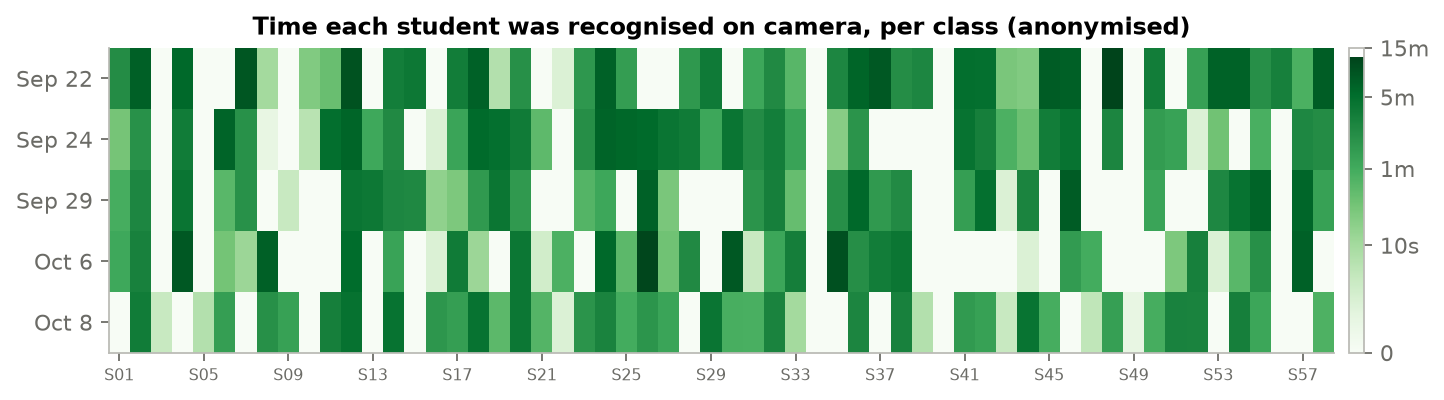
\includegraphics[width=0.9\textwidth]{figures/f06_attendance_matrix.png}
\caption{Time each student (anonymous id) was recognised on camera, per class.}\label{fig:attname}
\end{figure}

\end{document}
